\documentclass{article}
\usepackage[utf8]{inputenc}
\usepackage{graphicx}

\title{TUGAS BESAR DATABASE 2 \\     
Aplikasi Persediaan Obat}

\author{Dian Markuci (1184095)}
\date{December 2019}

\begin{document}

\maketitle

\section{Membuat Aplikasi Pada Oracle Express}
\subsection{Basis Data Oracle}
Basis data Oracle adalah basis data relasional yang 
terdiri dari kumpulan data dalam suatu sistem 
manajemen basis  data  RDBMS.Perusahaan 
perangkat lunak Oracle memasarkan jenis basis data 
ini untuk bermacam-macam aplikasi yang bisa 
berjalan  pada  banyak  jenis  dan  merk  perangkat 
keras komputer (platform). Oracle XE (Express Edition) adalah sebuah produk database server yang berlisensi freeware dari Oracle Corporation. Dengan produk ini, para pemakai Oracle XE dapat menggunakannya tidak hanya untuk percobaan, tetapi juga dapat digunakan untuk pengembangan dan deployment sistem. 

\subsection{Langkah-langkah membuat Aplikasi}
syarat utamanya adalah sudah memiliki akun oracle untuk login. setelah sukses login maka tampilannya akan seperti ini :

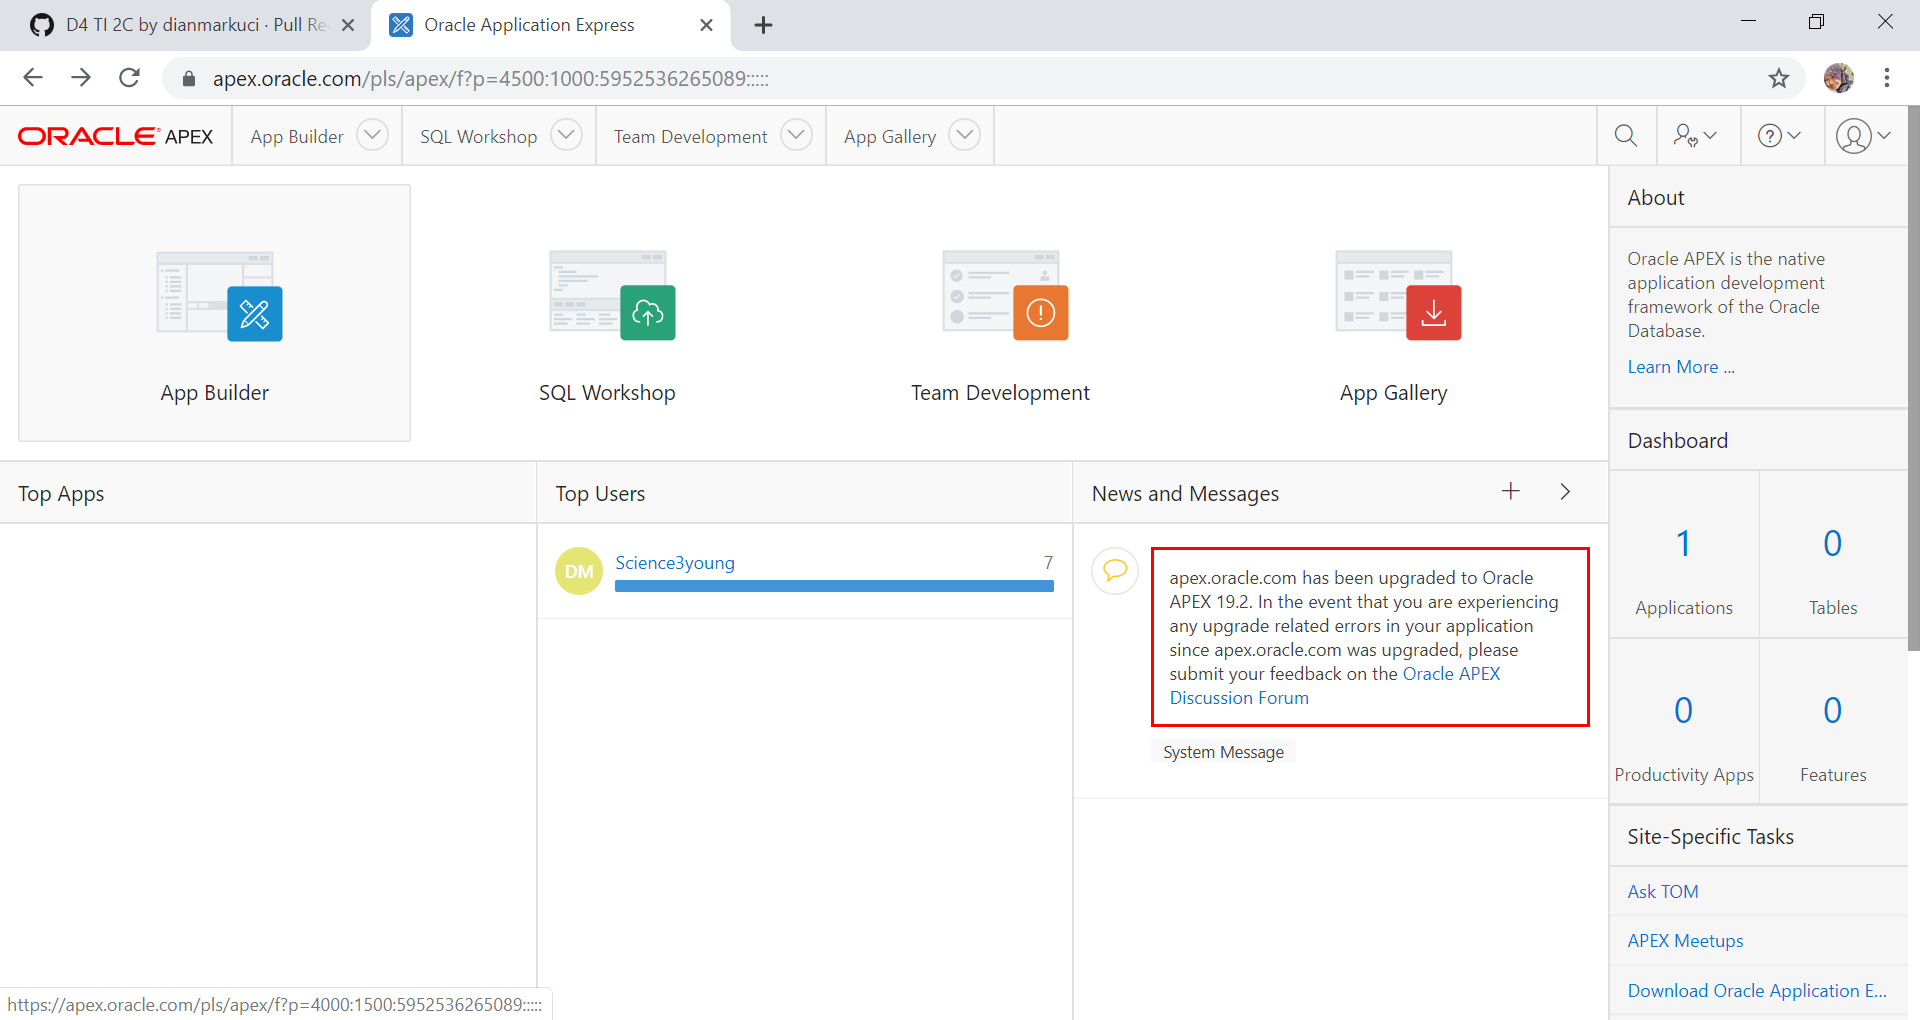
\includegraphics[width=13cm]{figure/1.png}
gambar diatas merupakan tampilan utama sebuah workspace, dimana kita bisa membuat aplikasi menggunakan menu app builder, menu sql workshop, objek browser untuk melihat tabel, skema, view dan komponen lain dalam database. didalam menu sql ini juga ada sql commands yaitu sebuah tempat untuk membuat komponen-komponen didalam database menggunakan \textit{Querry SQL}. di apex juga terdapat menu Saved SQL dimana Saved SQL ini memudahkan kita untuk menyimpan querry sql apabila suatu saat kita membutuhkan querry tersebut. 

Langsung saja membuat querry sql di sql commands. Untuk aplikasinya sendiri, saya menggunakan Aplikasi-Persediaan-Obat. dimana ada 2 tabel Obat dan Obat Masuk dimana pada tabel obat terdiri dari kode obat, nama obat, harga beli dan harga jual, sedangkan obat masuk terdiri dari kode transaksi, tanggal masuk, kode obat, dan jumlah masuk. Berikut langkahnya :

\begin{enumerate}
    \item Memasukkan Querry Pertama : CREATE TABLE 
\end{enumerate}

\begin{center}
    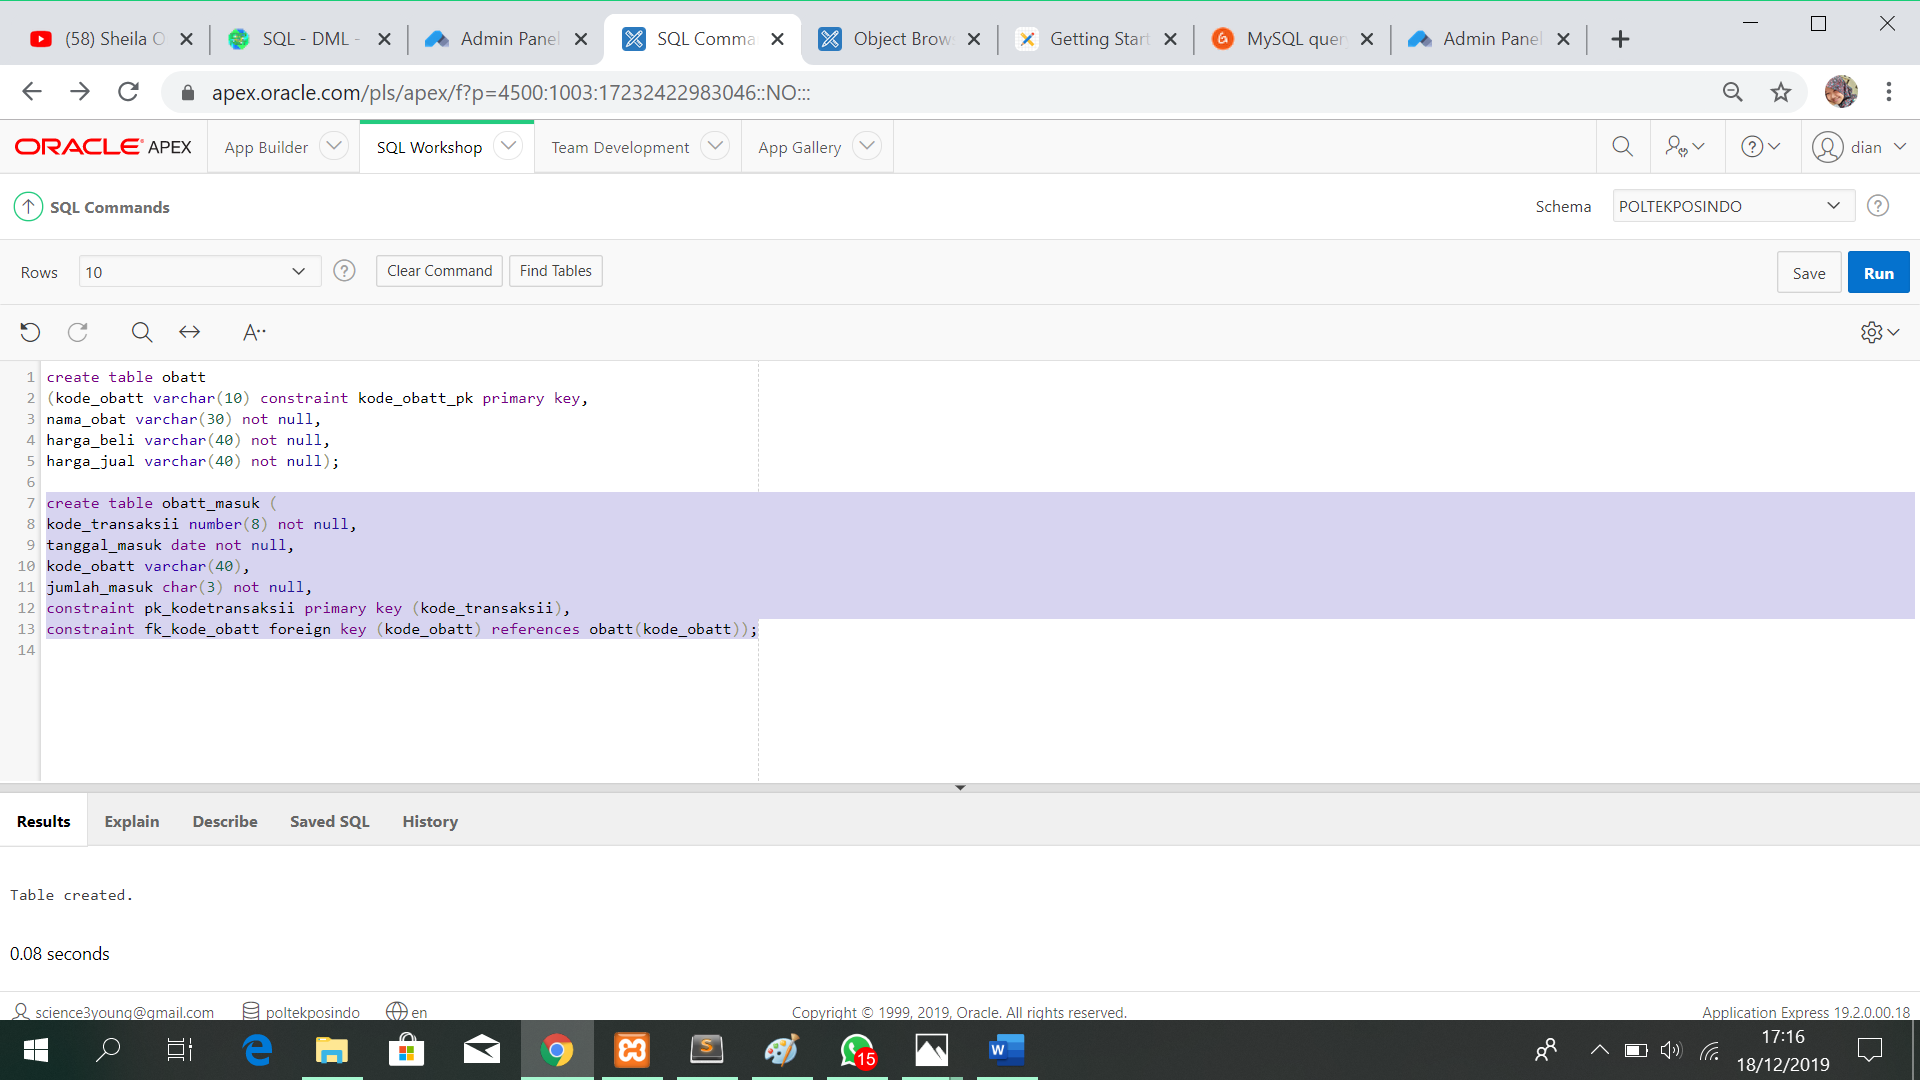
\includegraphics[width=13cm]{figure/tabelbaru2.png}
\end{center}

CREATE TABLE (masukkan nama tabelnya), untuk baris bawahnya adalah nama dari kolom yang terdapat pada tabel. varchar,date,int merupakan nama type datanya, (15), (30) dll merupakan panjang data yang dapat diisikan kedalam masing-masing kolom. Not Null artinya kolom yang tidak boleh kosong. Setelah itu block kemudian RUN maka ketika berhasil dibuat akan ada hasil/ result \textit{table created 0,.. seconds}\\


     2. Memasukkan Querry Kedua : INSERT TABLE\\


\begin{center}
    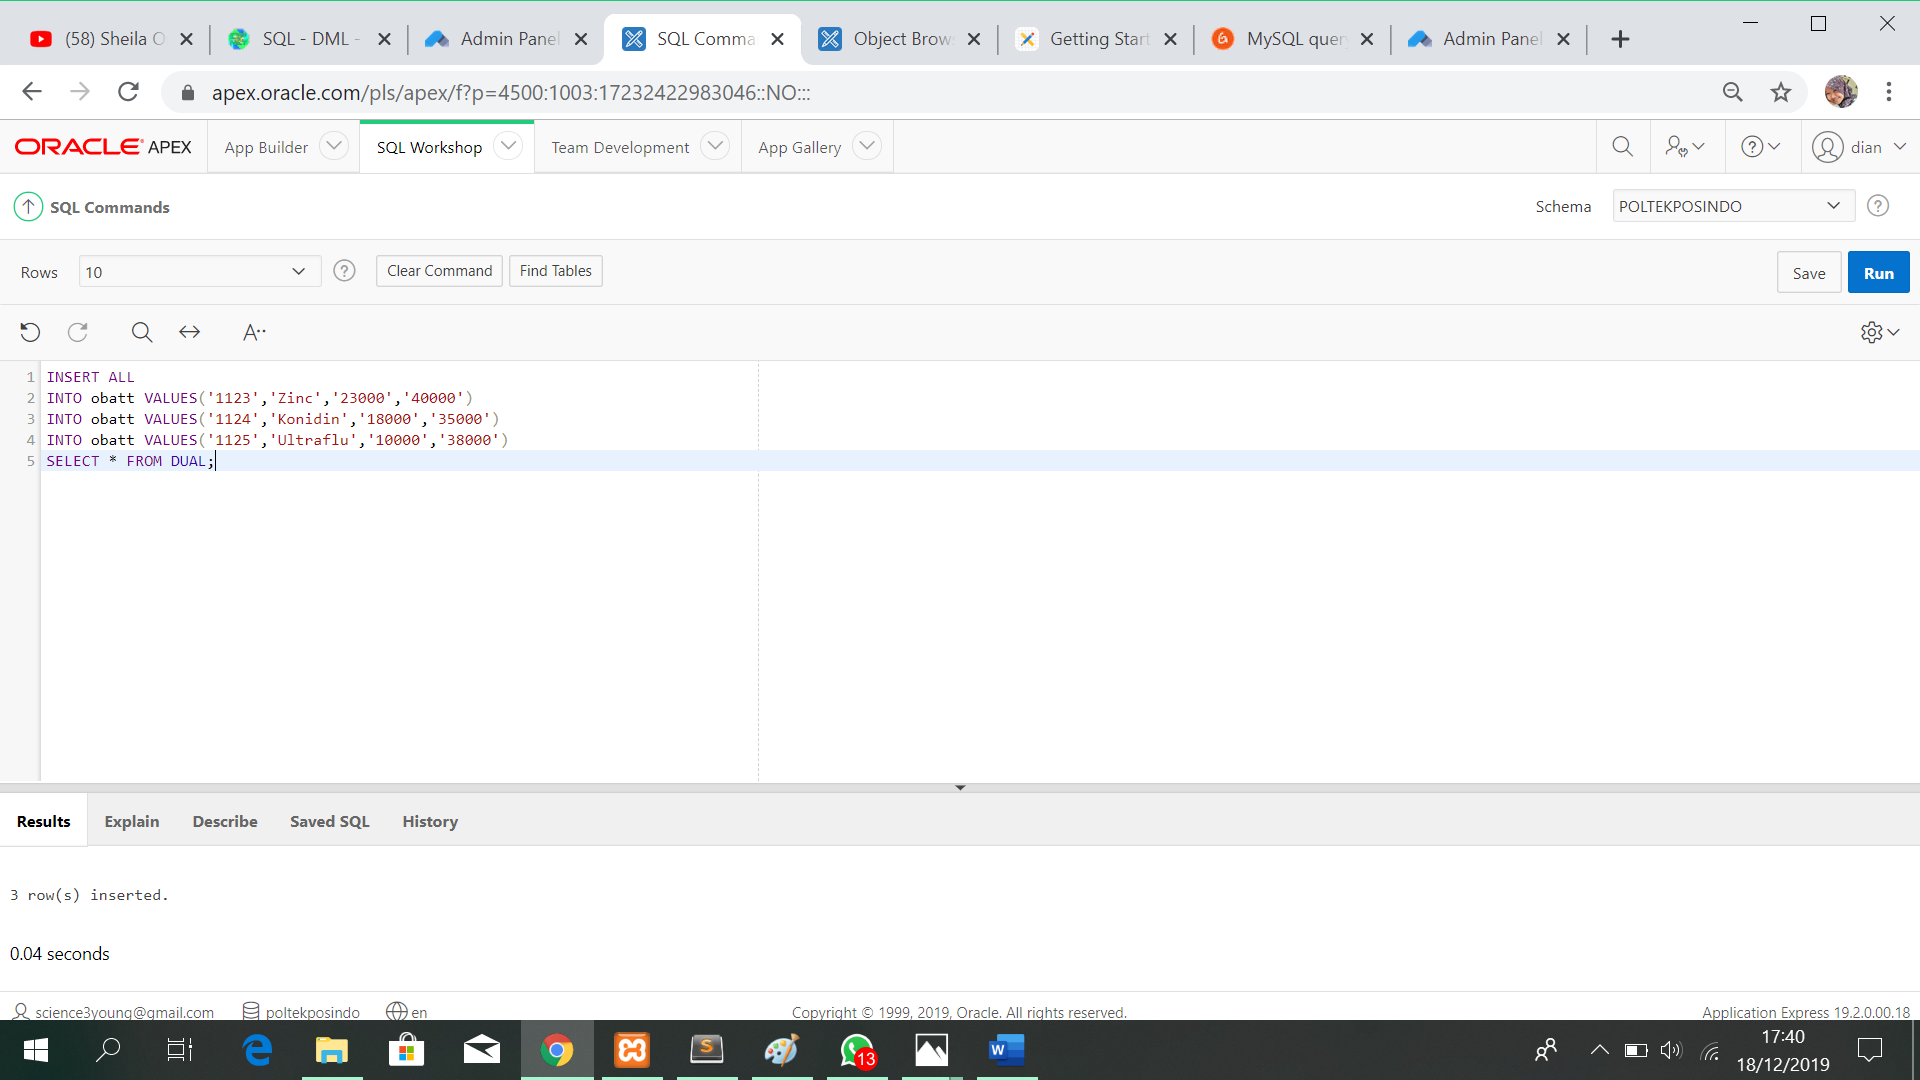
\includegraphics[width=13cm]{figure/insert1.png}
    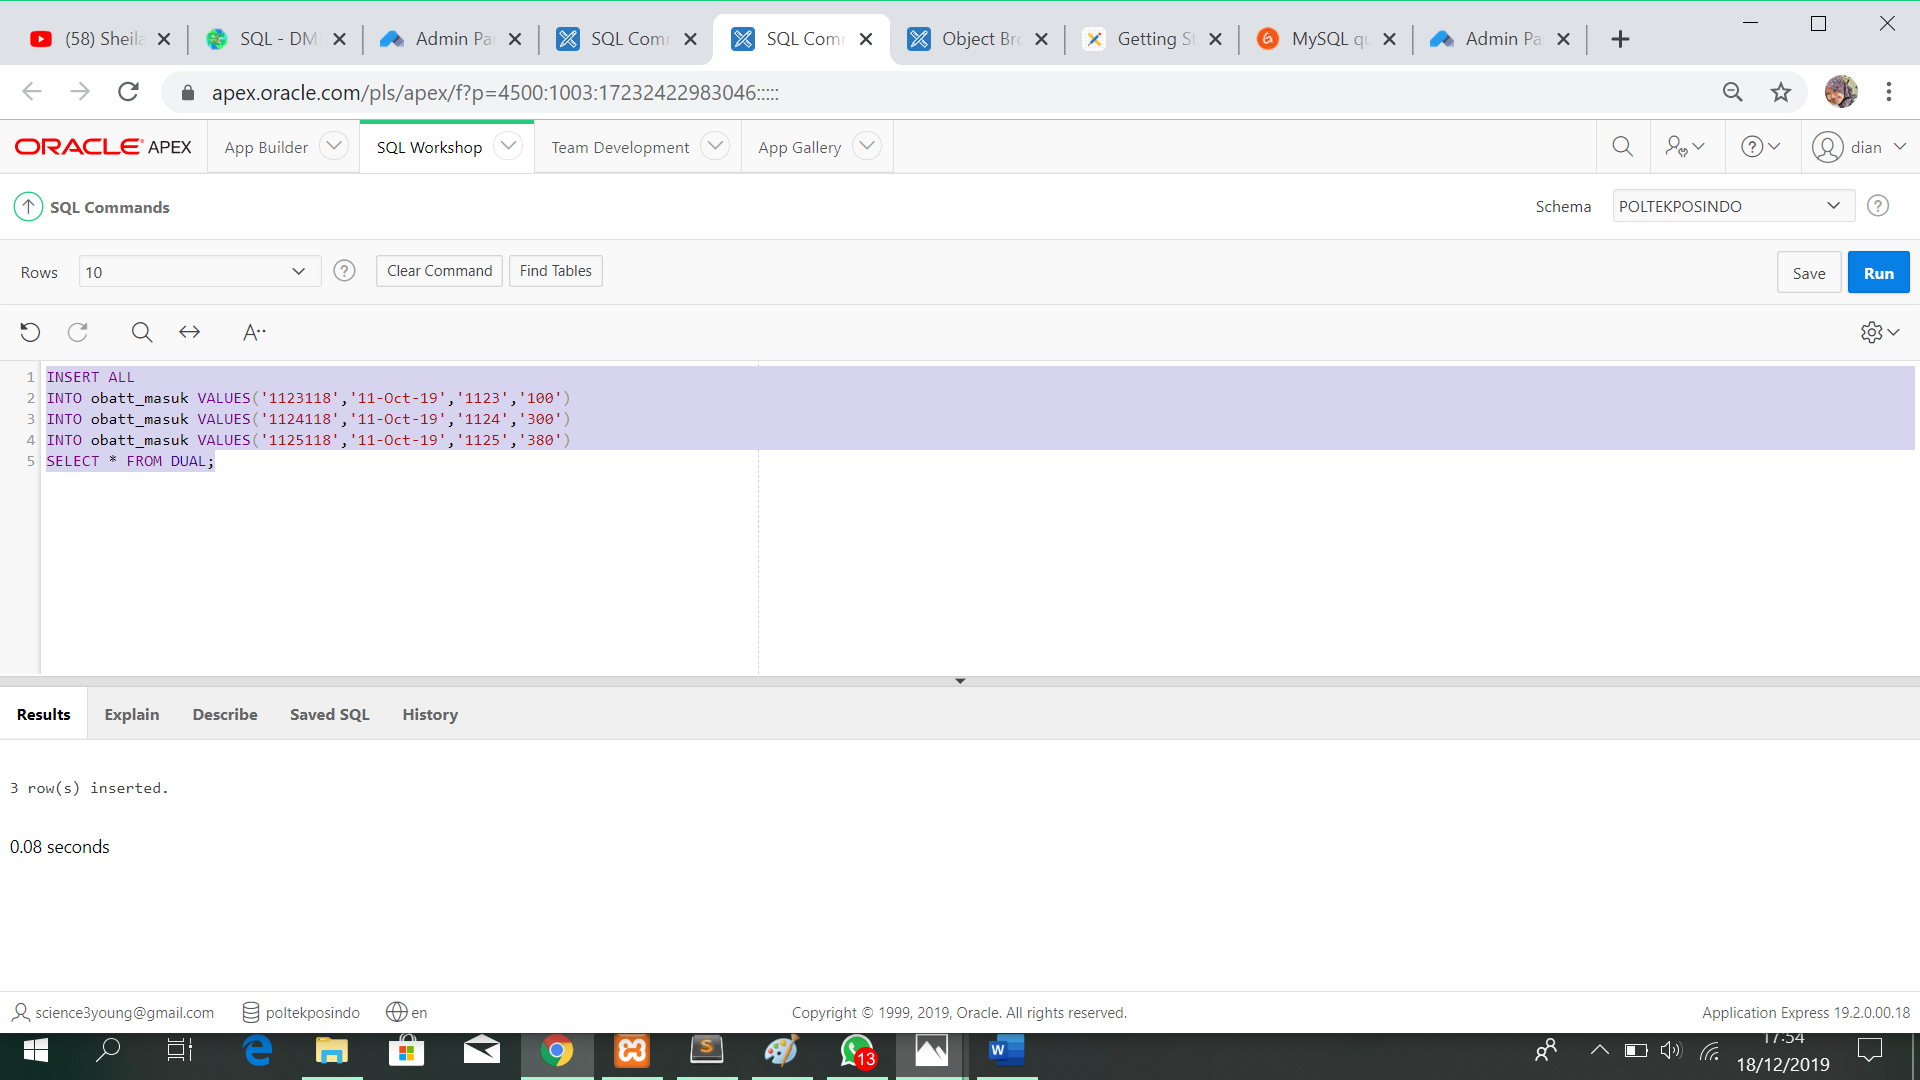
\includegraphics[width=13cm]{figure/insert2.png}
\end{center}

setelah table berhasil dibuat maka akan dicoba menginsertkan data pada table yang sudah dibuat. caranya bisa satu persatu ataupun secara sekaligus. untuk yang sekaligus menggunakan perintah INSERT dengan ditambahkan ALL dan dibawahnya ketikkan perintan INTO (nama table) values(isi table) setelah di run dan berhasil maka akan ada hasil .. rows(s) inserted 0,.. seconds)\\

    3. Implementasikan FUNGSI TRIGGER DAN VIEW\\

Dalam DBMS (Database Management System), trigger merupakan kumpulan script yang berhubungan dengan table, view ataupun skema yang dijalankan secara otomatis ketika terdapat event yang dijalankan. Event tersebut meliputi operasi yang biasa dilakukan dalam mengolah database, seperti : 

\begin{enumerate}
    \item DML (Data Manipulation Language) yang meliputi DELETE, INSERT atau UPDATE
    \item DDL (Data Definition Language) yang meliputi CREATE, ALTER atau DROP
    \item Operasi Database lainnya, seperti SERVERERROR, LOGON, LOGOFF, STARTUP atau SHUTDOWN)
\end{enumerate}

langkah implementasi :\\
1. membuat trigger dengan nama trigger yang dibuat sesuai dengan karakteristik penamaan dalam MySQL. namun sebelumnya membuat table history obat sebelum membuat trigger. nama table : menunjukkan table yang akan dilakukan trigger didalamnya. \\

\begin{center}
    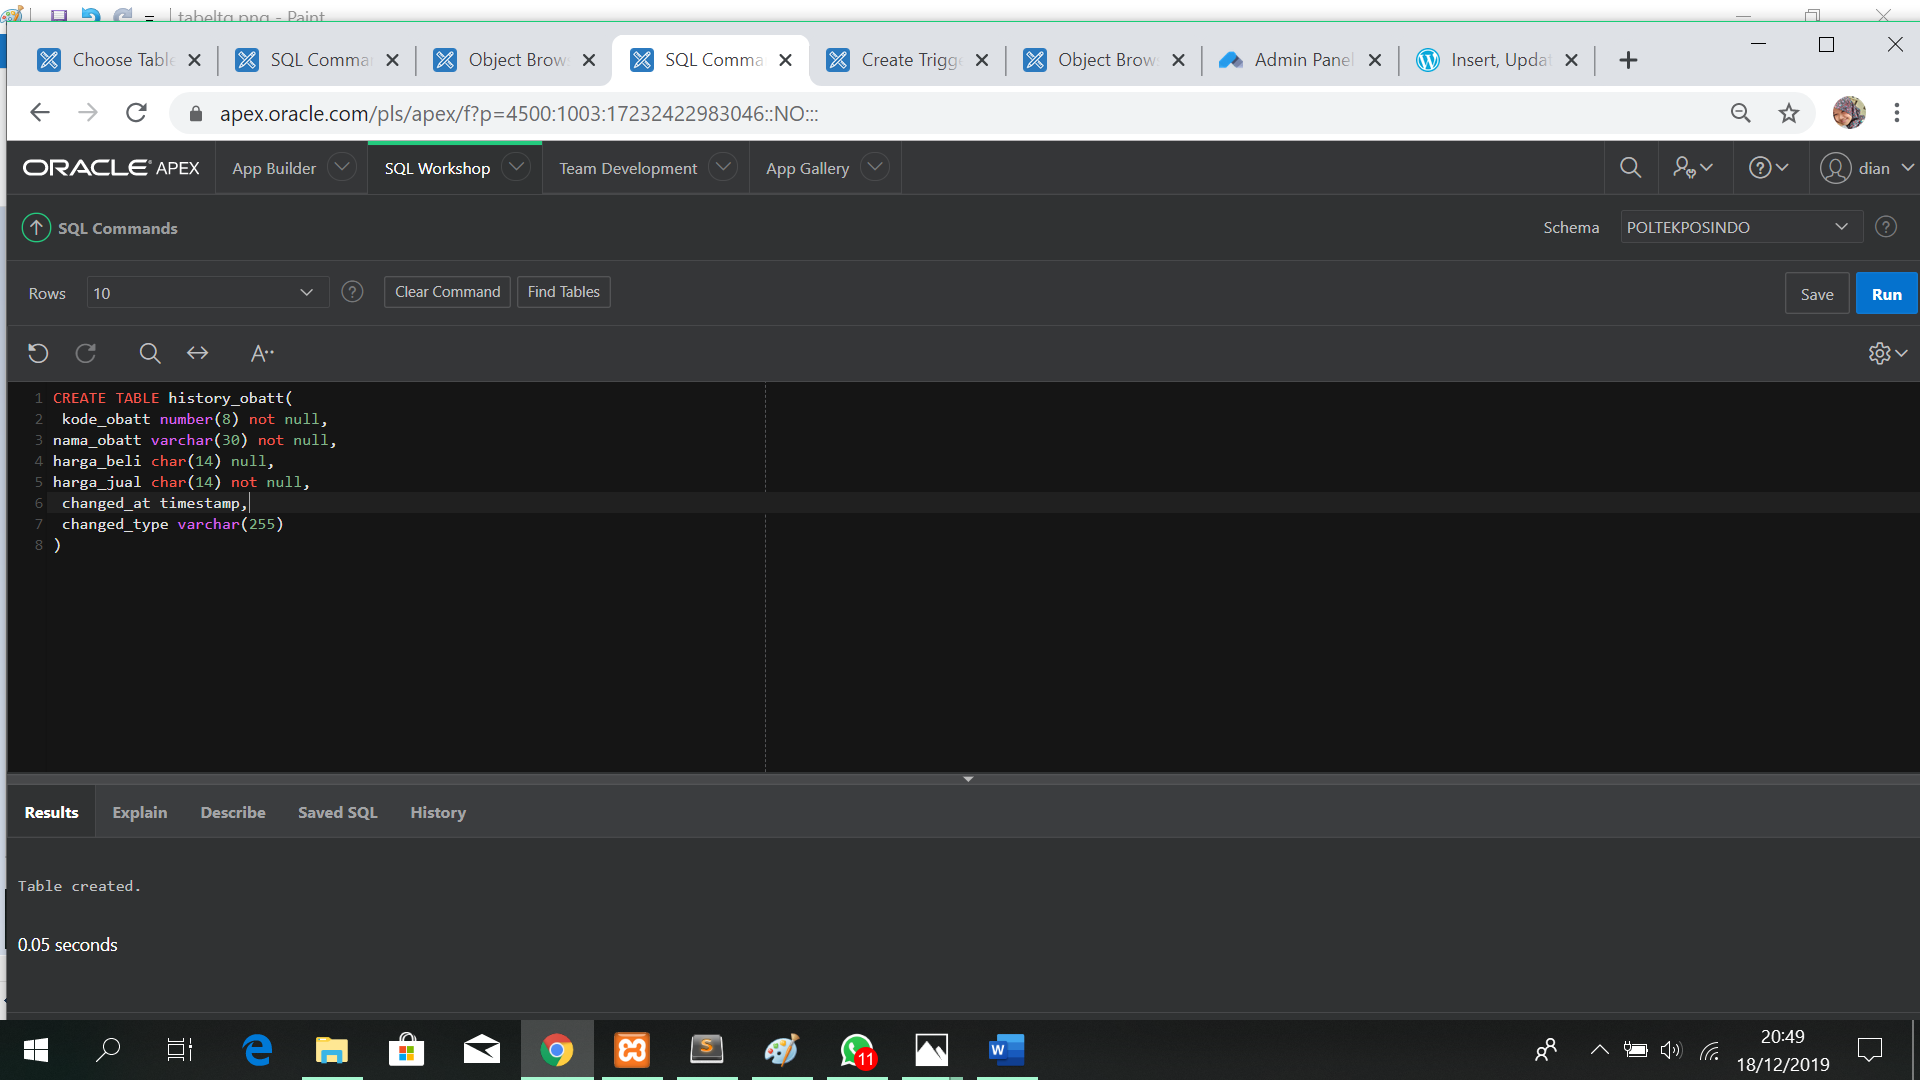
\includegraphics[width=13cm]{figure/tablehistory.png}
\end{center}

\textit {sebelumnya tampilan diatas menggunakan dark mode}\\

2. Membuat Trigger (Insert, Update, dan Delete)

\begin{center}
    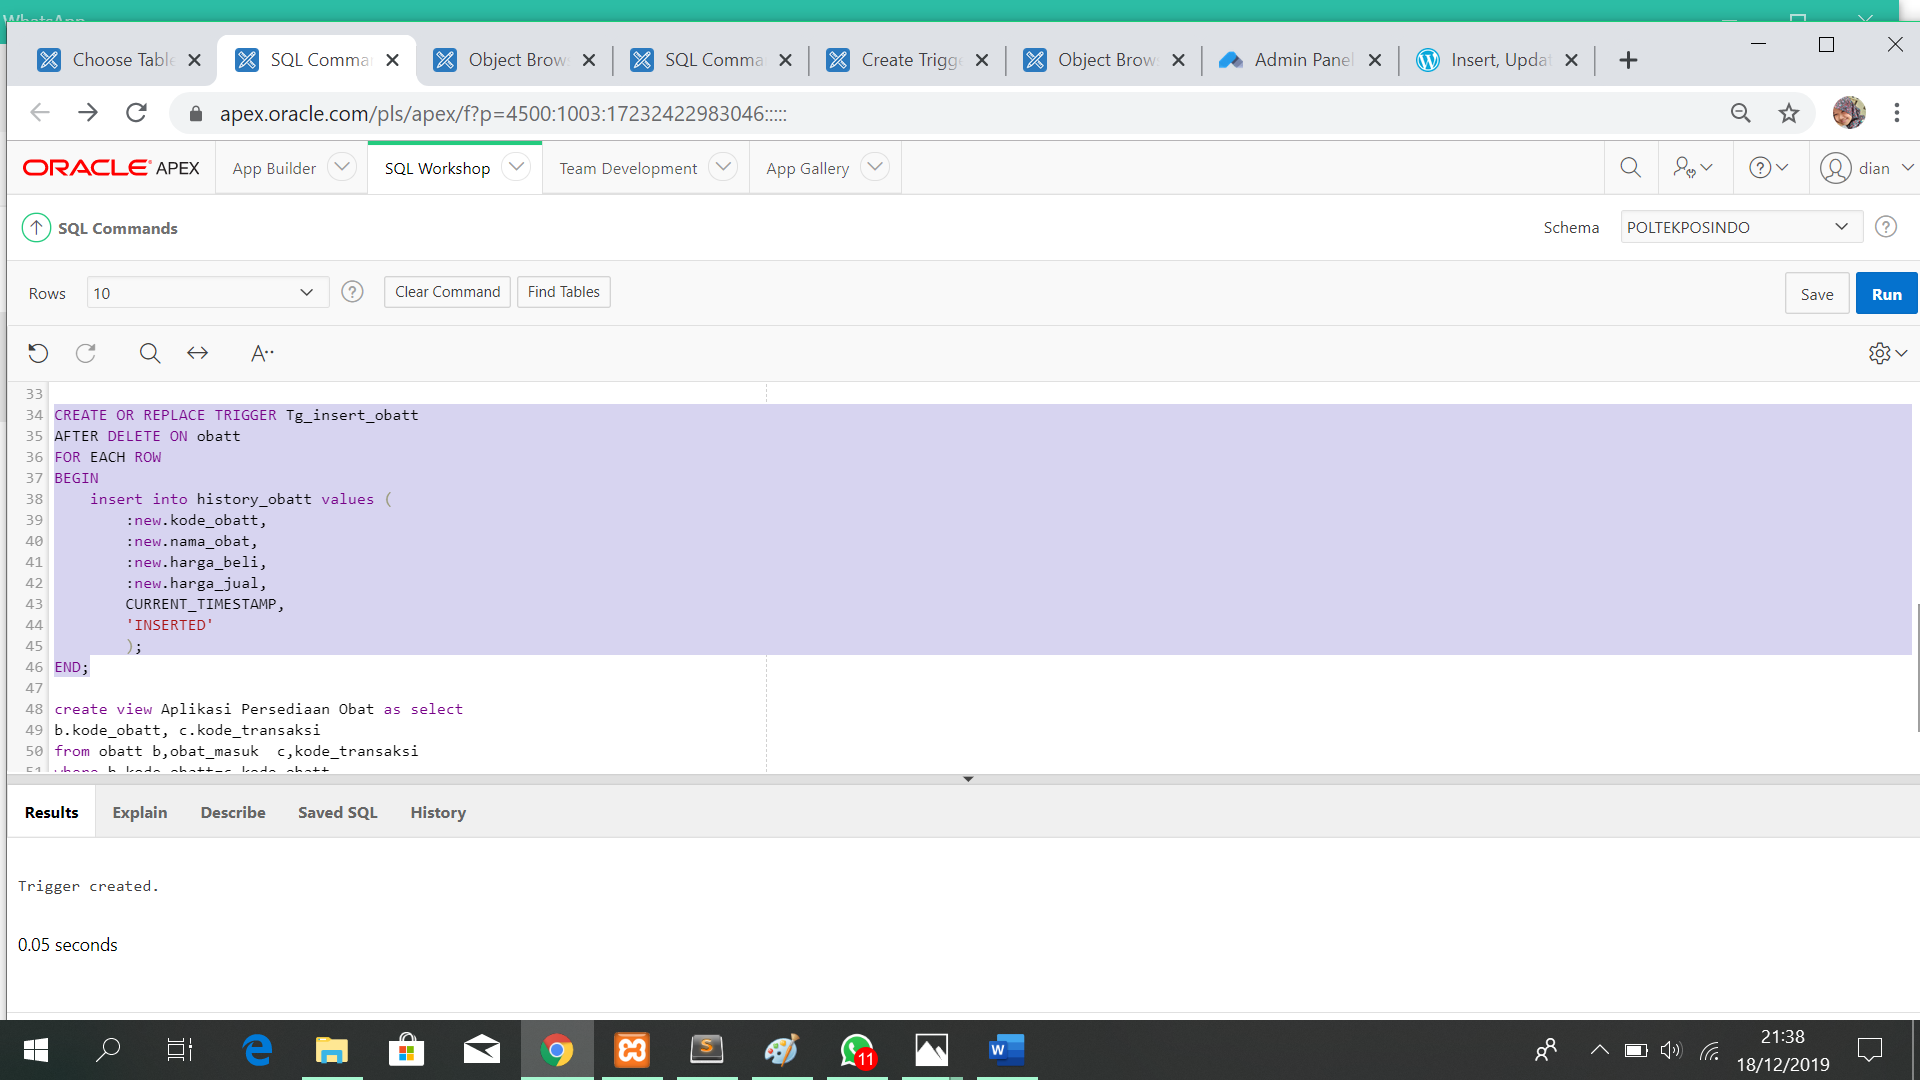
\includegraphics[width=13cm]{figure/tginserted.png}
    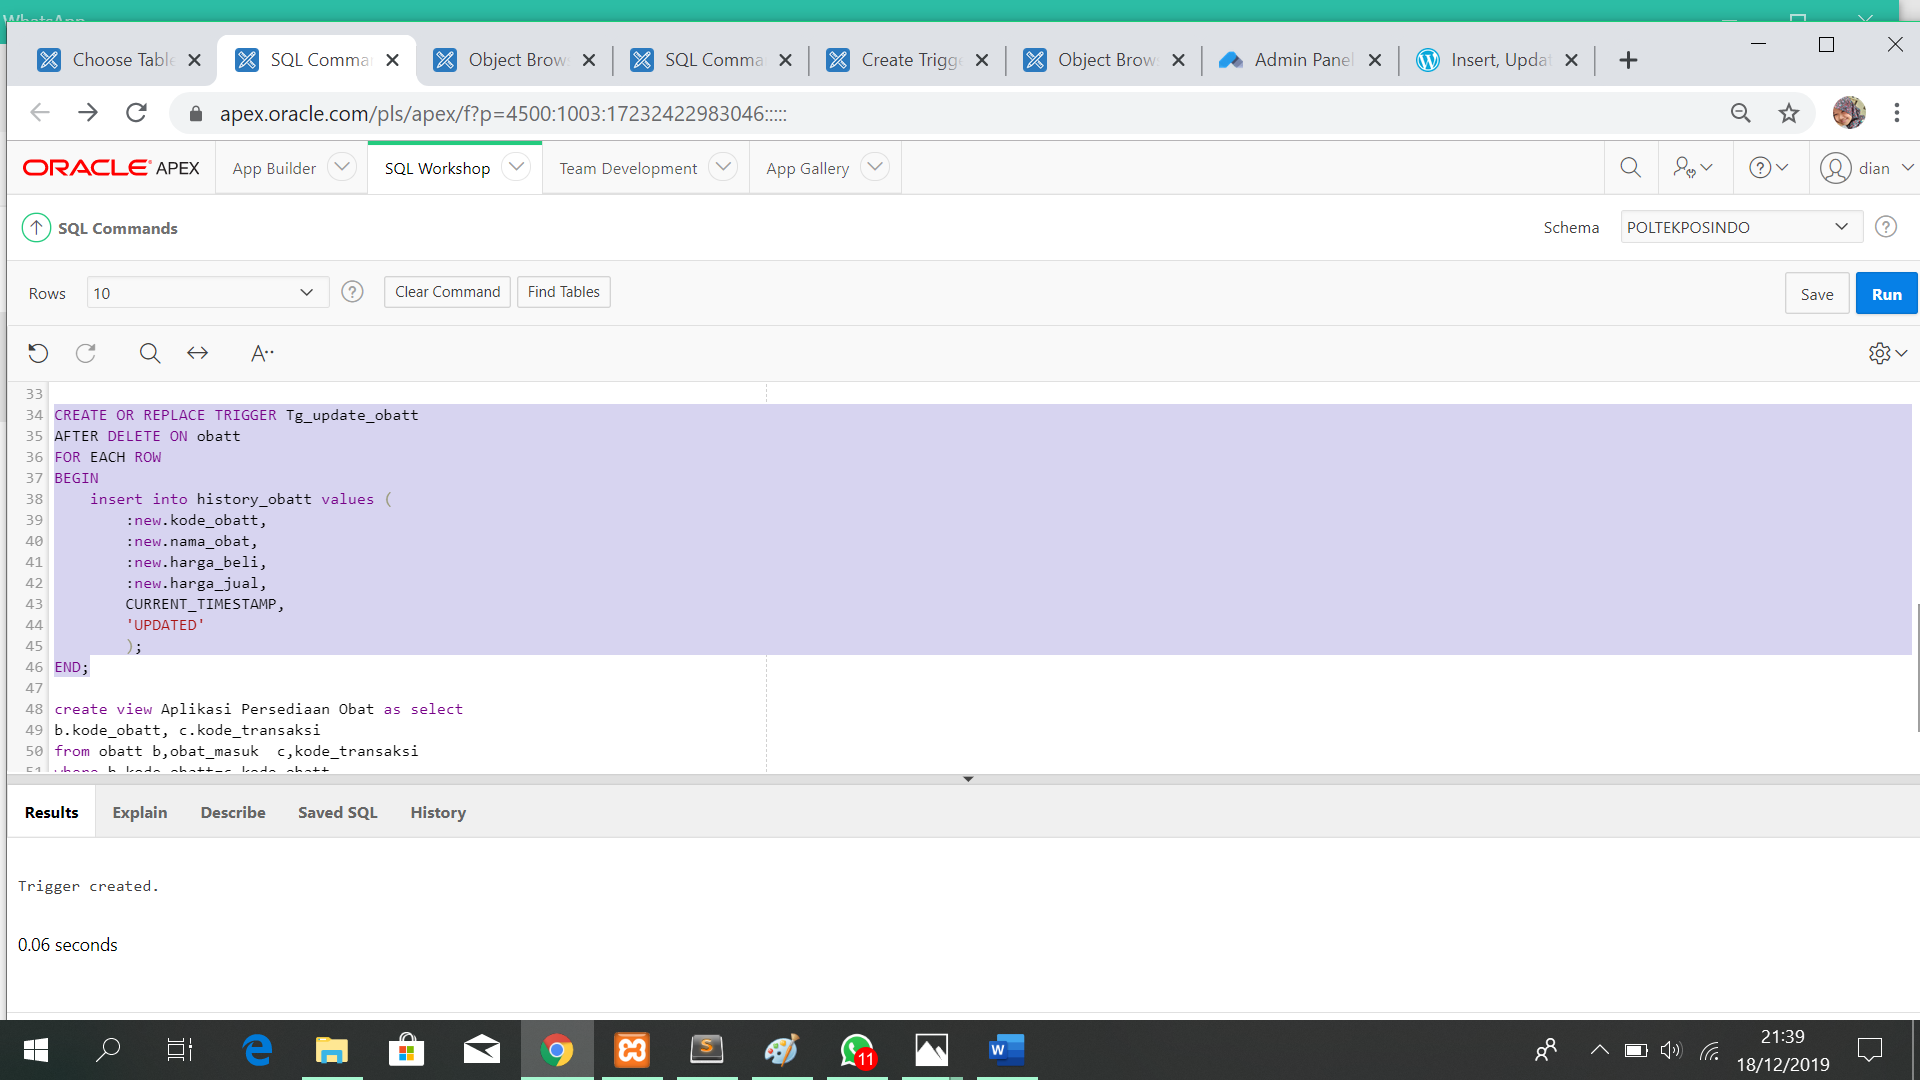
\includegraphics[width=13cm]{figure/TGUPDATE.png}
    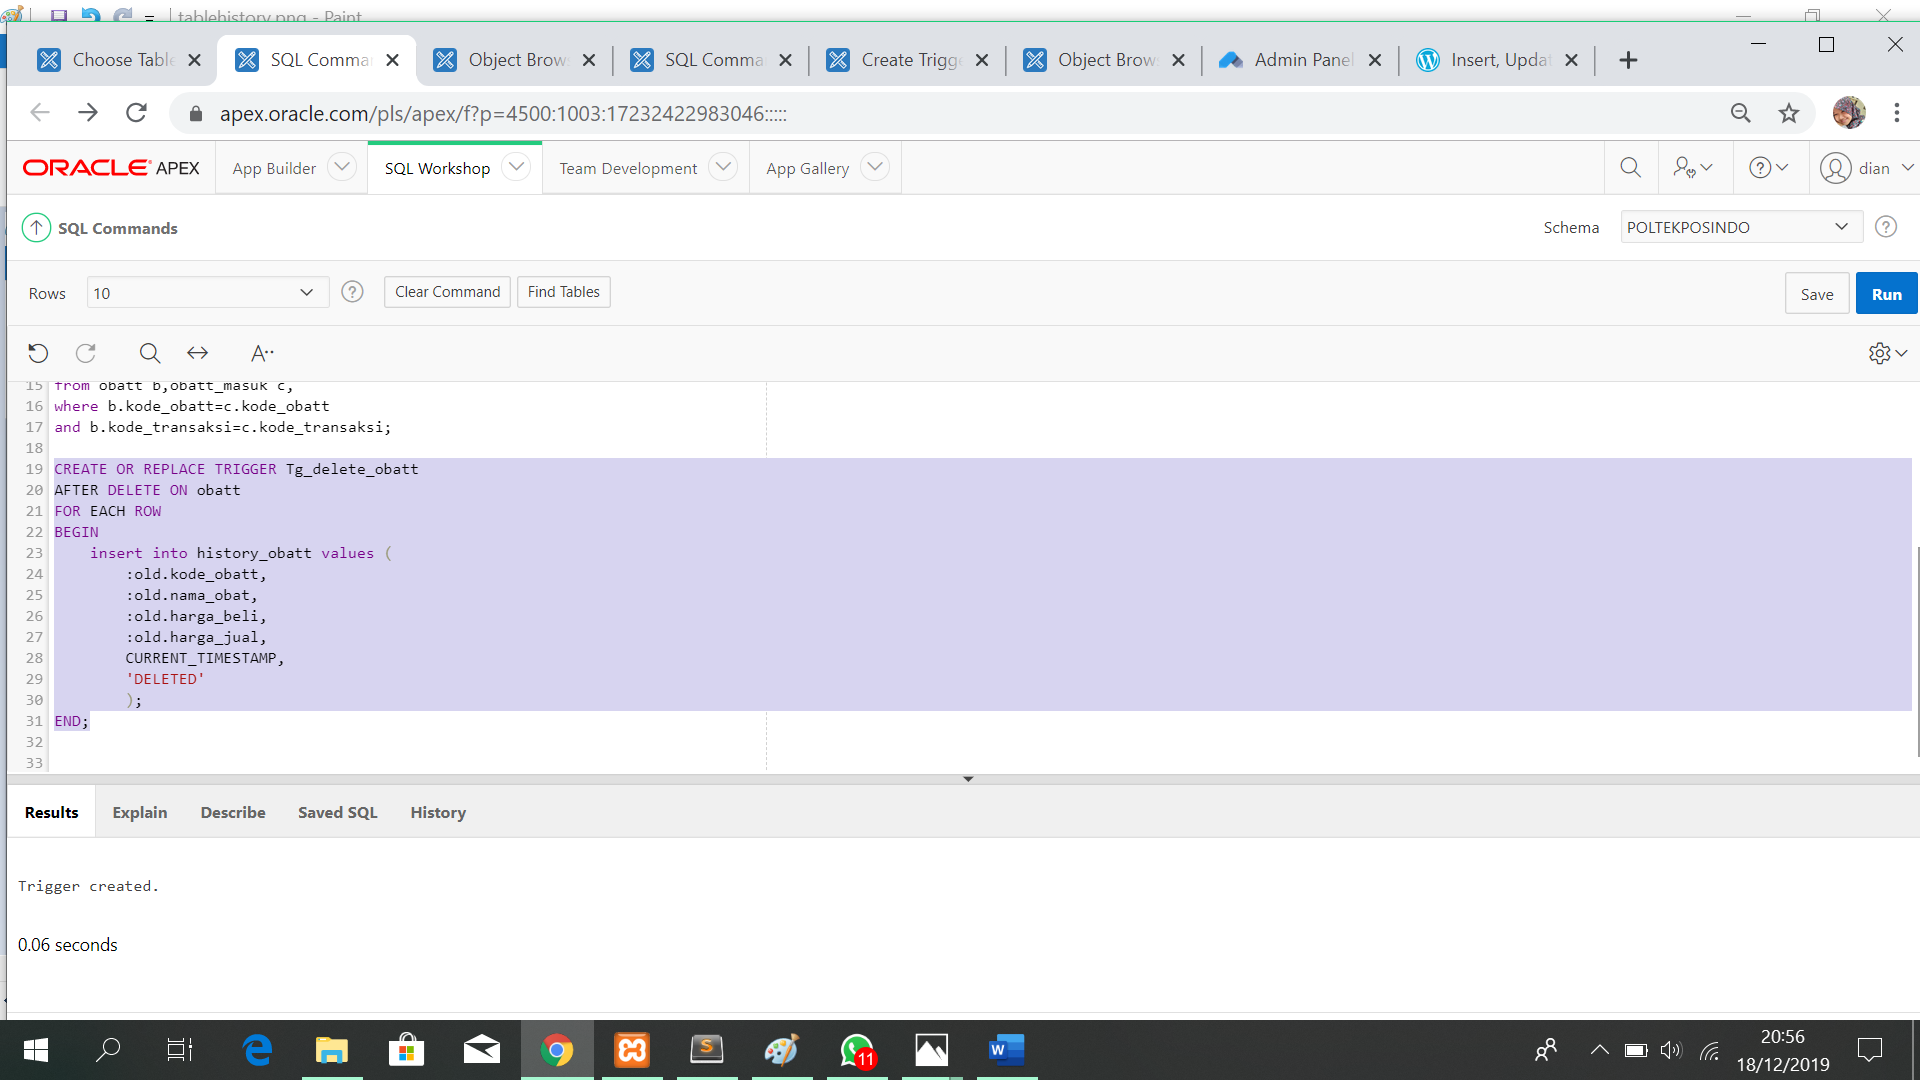
\includegraphics[width=13cm]{figure/triggercreated.png}
\end{center}

(INSERT , UPDATE , DELETE) : digunakan untuk menentukan event yang menyebabkan terjadinya trigger, pilihan event tersebut terdiri dari INSERT, UPDATE dan DELETE.
\\
Sedangkan Fungsi View, SQL view digunakan untuk membuat tampilan sebuah tabel. Di dalamnya memungkinkan kita untuk bisa membuat, mengupdate dan menghapus tampilan tabel tersebut. Dan tabel yang ditampilkan merupakan tabel hasil dari perintah-perintah MySql.
Untuk membuat View kita menggunakan perintah \textit{CREATE VIEW} dengan bentuk sbb:\\
\\CREATE VIEW namaview AS\\
SELECT namakolom\\
FROM namatabel\\
WHERE persyaratan\\
\\
    4. Tahap Pembuatan Aplikasi\\

1. Kembali ke Menu Utama, kemudian pilih APP BUILDER, Pilih CREATE
\begin{center}
    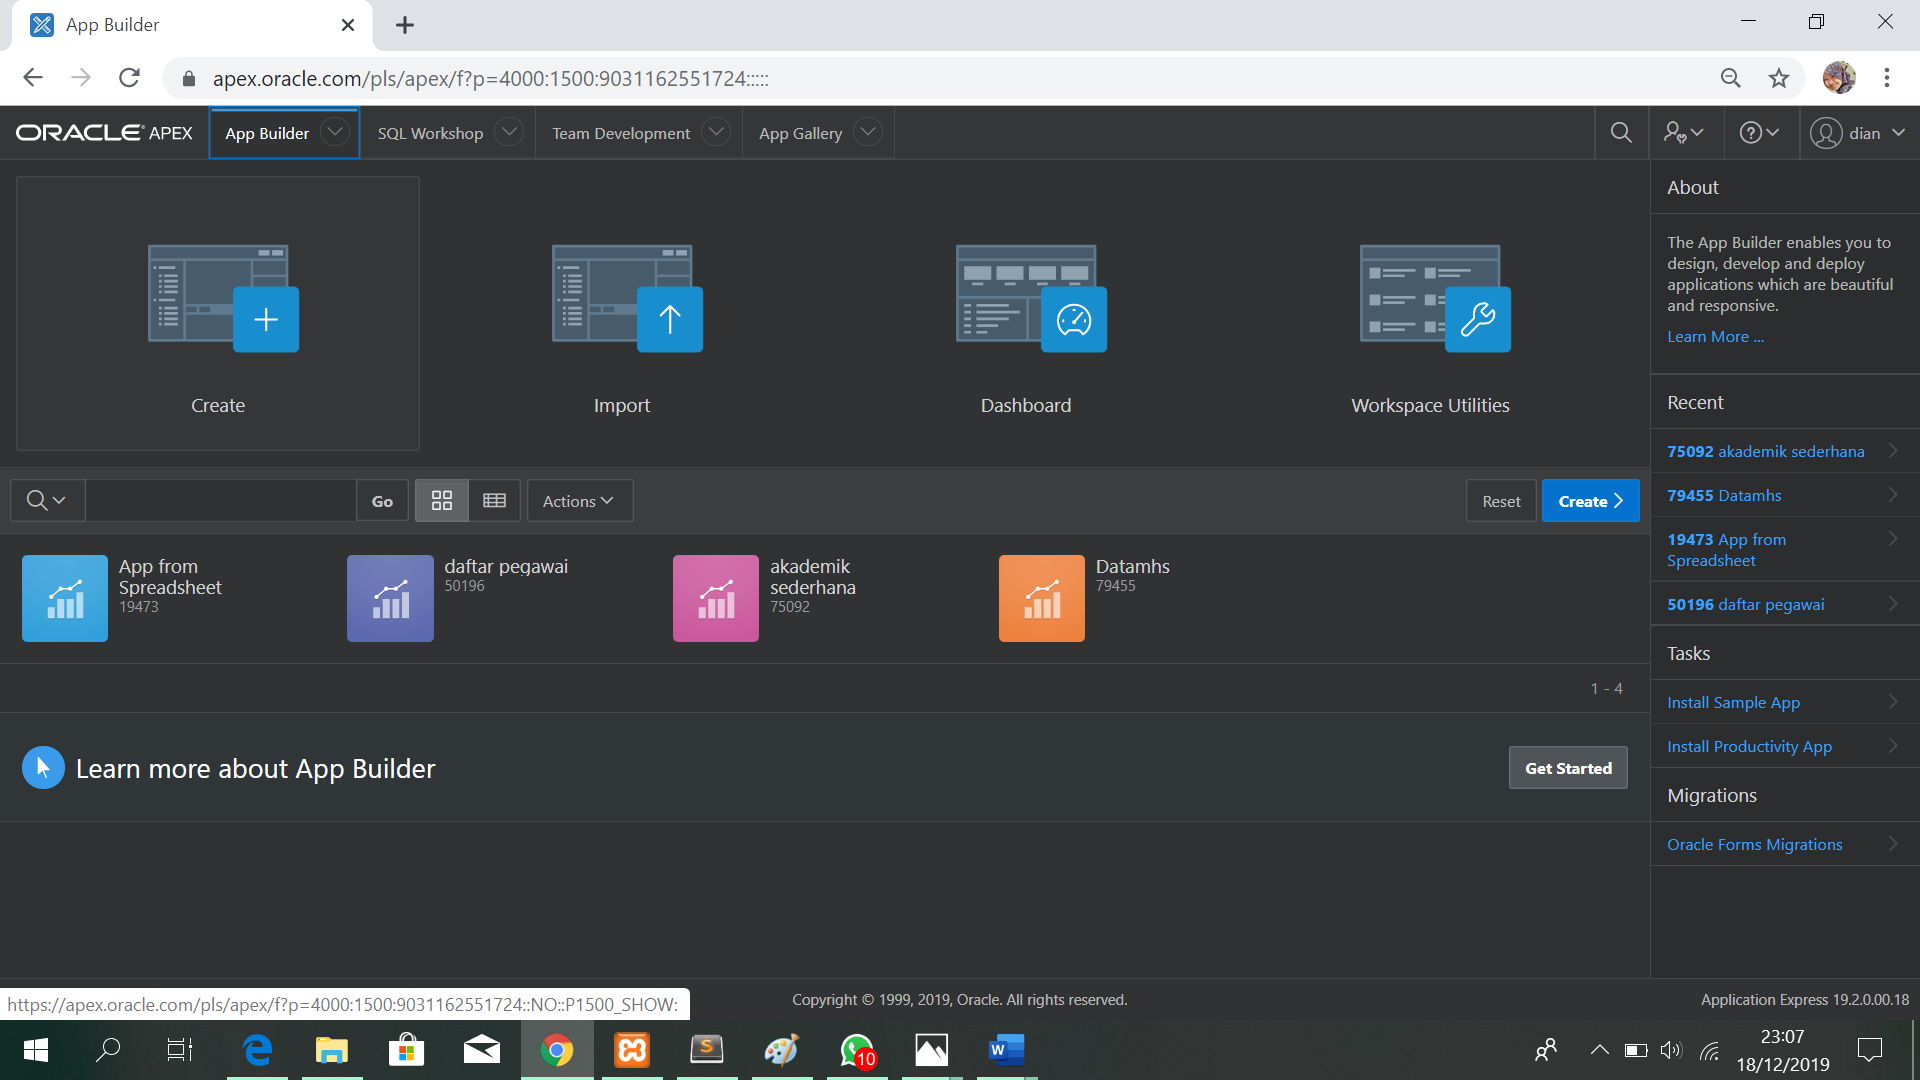
\includegraphics[width=13cm]{1.png}
\end{center}
\\
2. kemudian pilih NEW APPLICATION
\begin{center}
    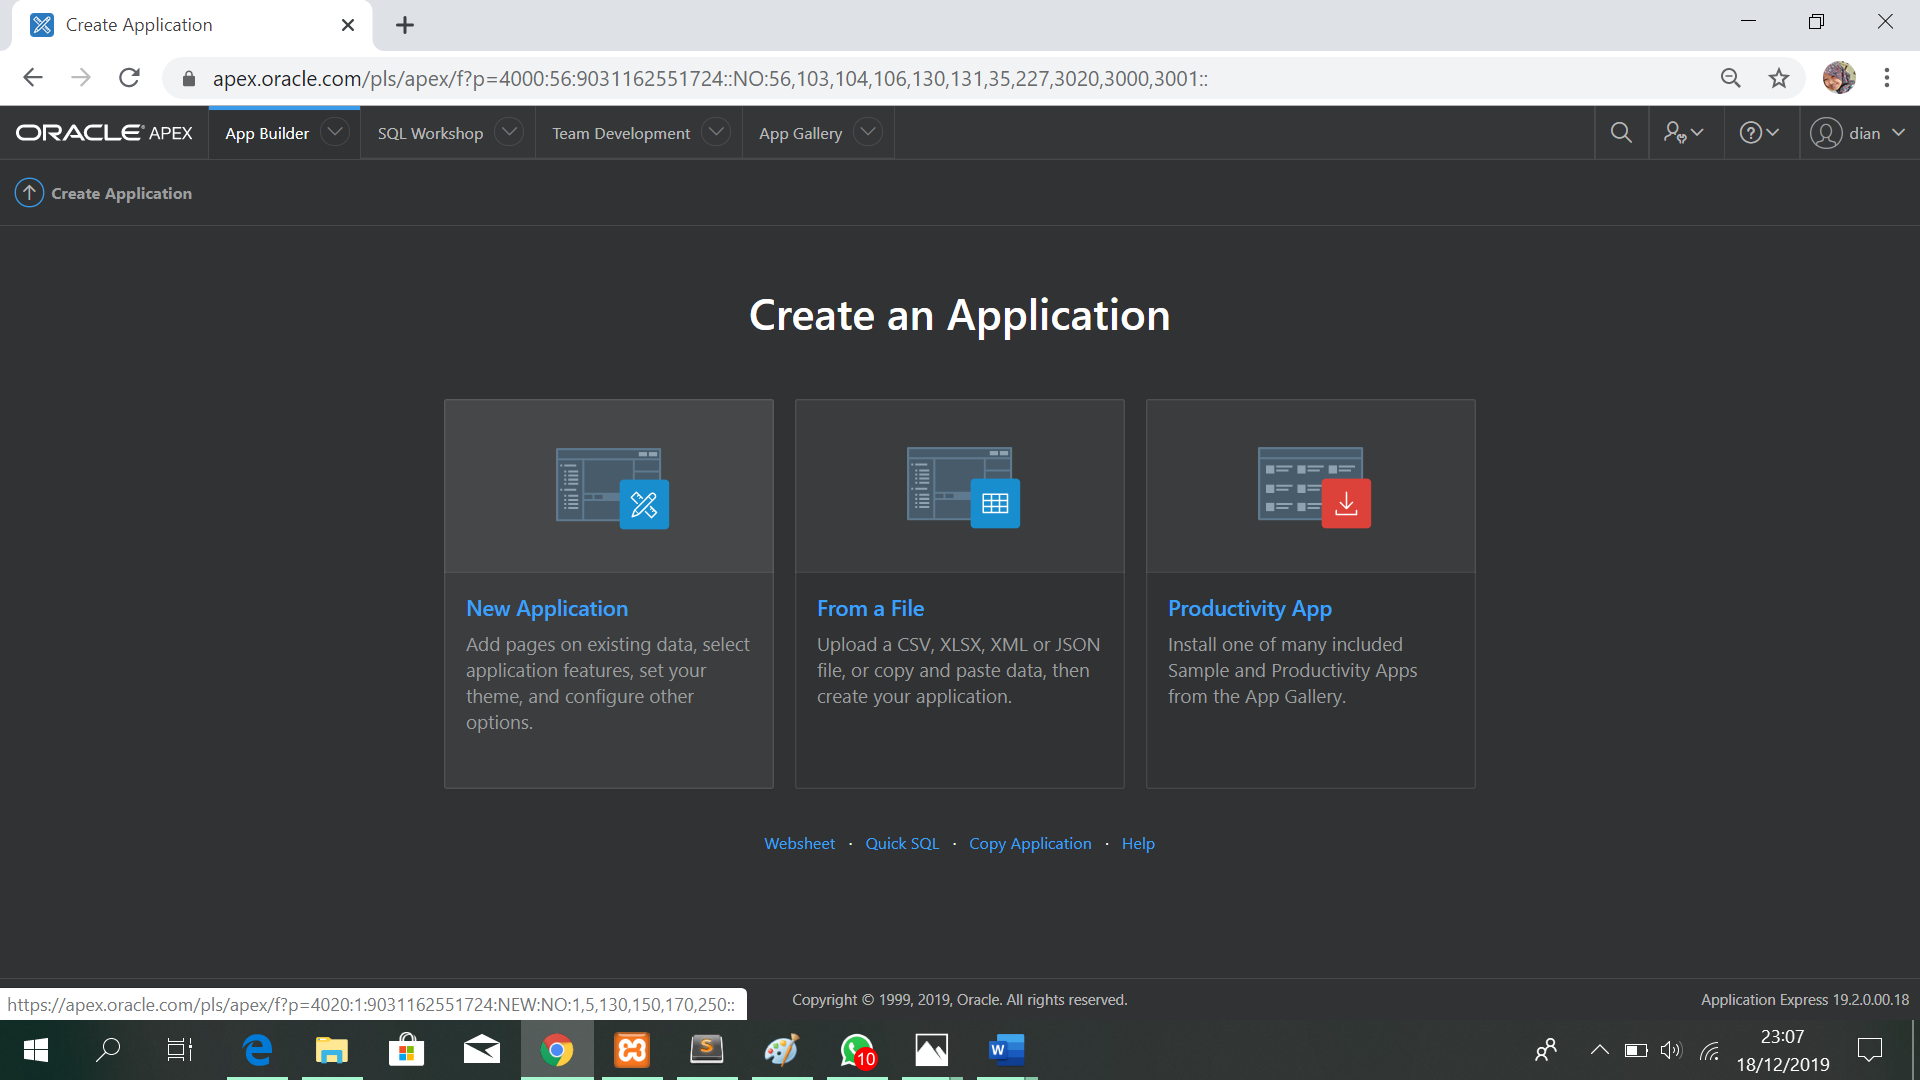
\includegraphics[width=13cm]{figure/2.png}
\end{center}
\\
3. Setelah itu Di Halaman Create an application. Ketikkan nama dan pages. Pilih add pages kemudian pilih forms.
\begin{center}
    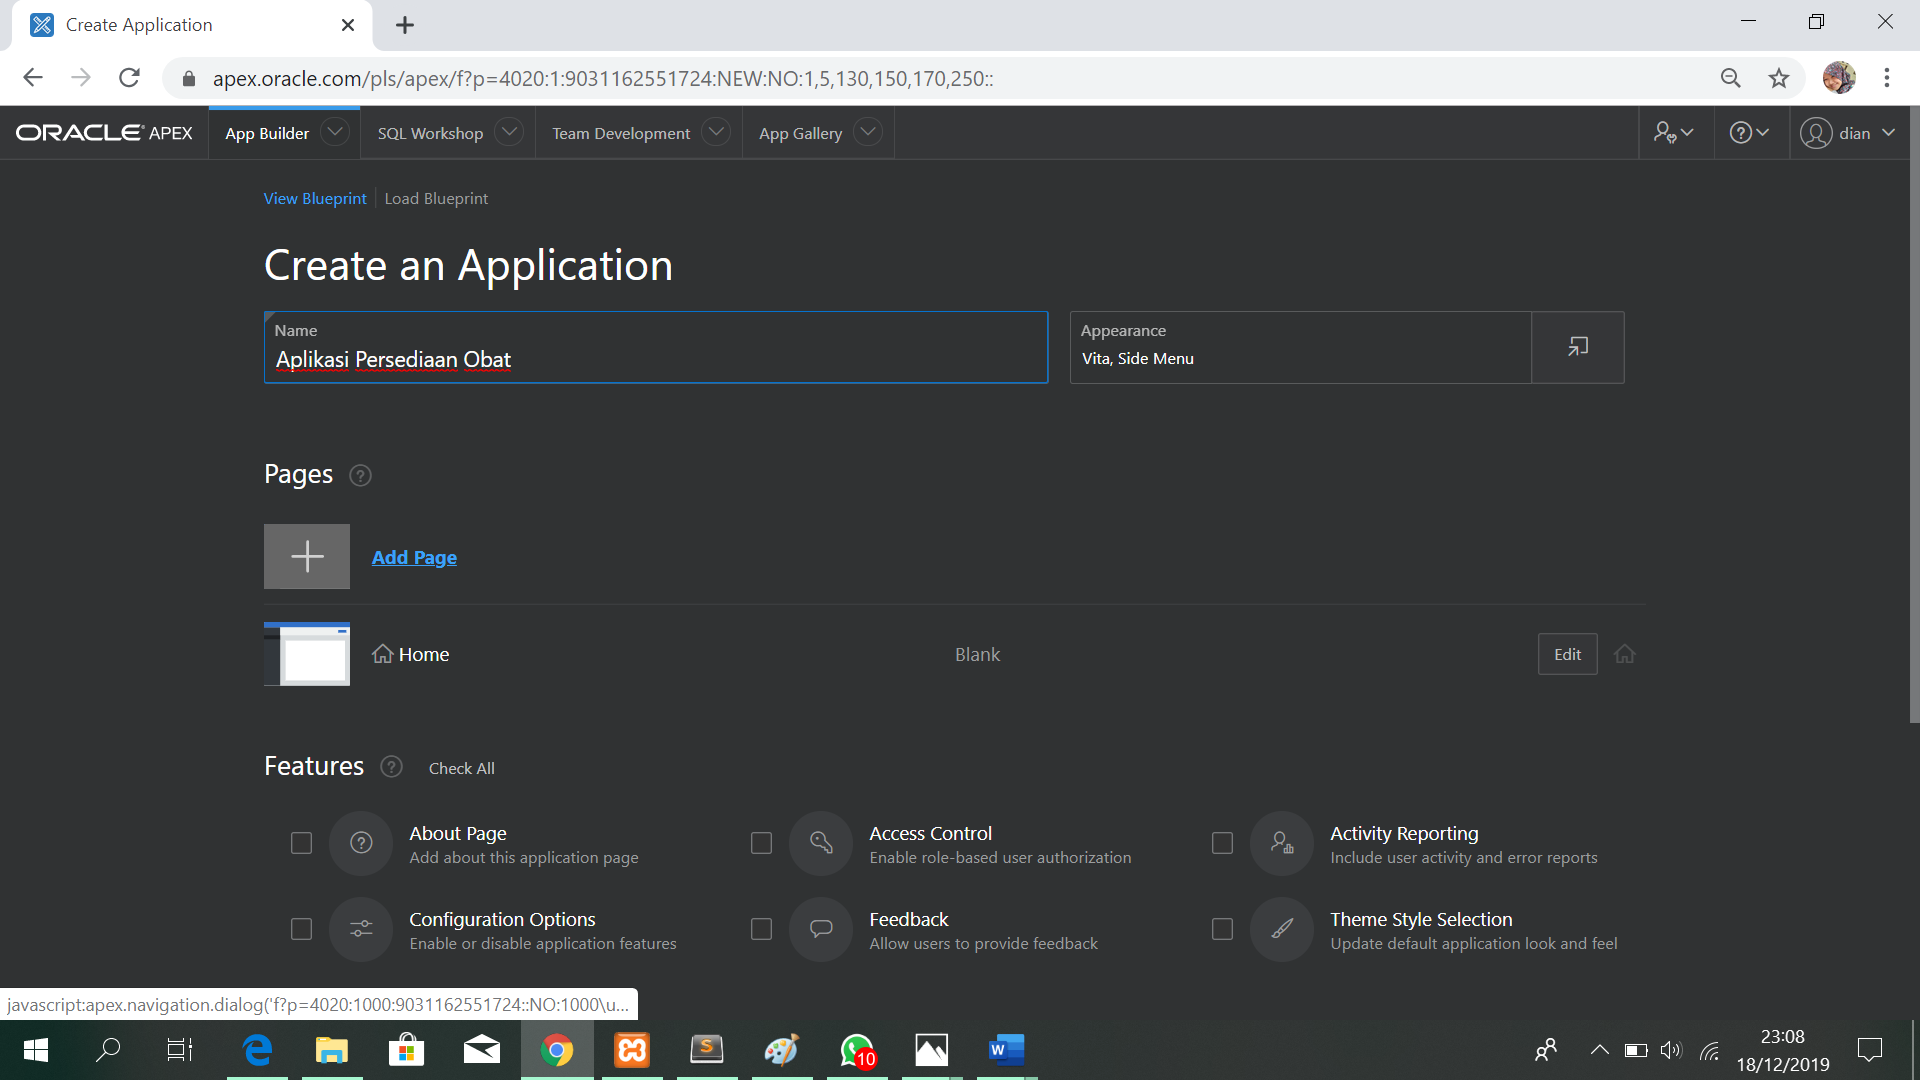
\includegraphics[width=13cm]{figure/3.png}
\end{center}
\\
4. Pada Halaman Create Form Page, ketikkan Page name, dan nama table yang sudah dibuat, kemudian klik add page
\begin{center}
    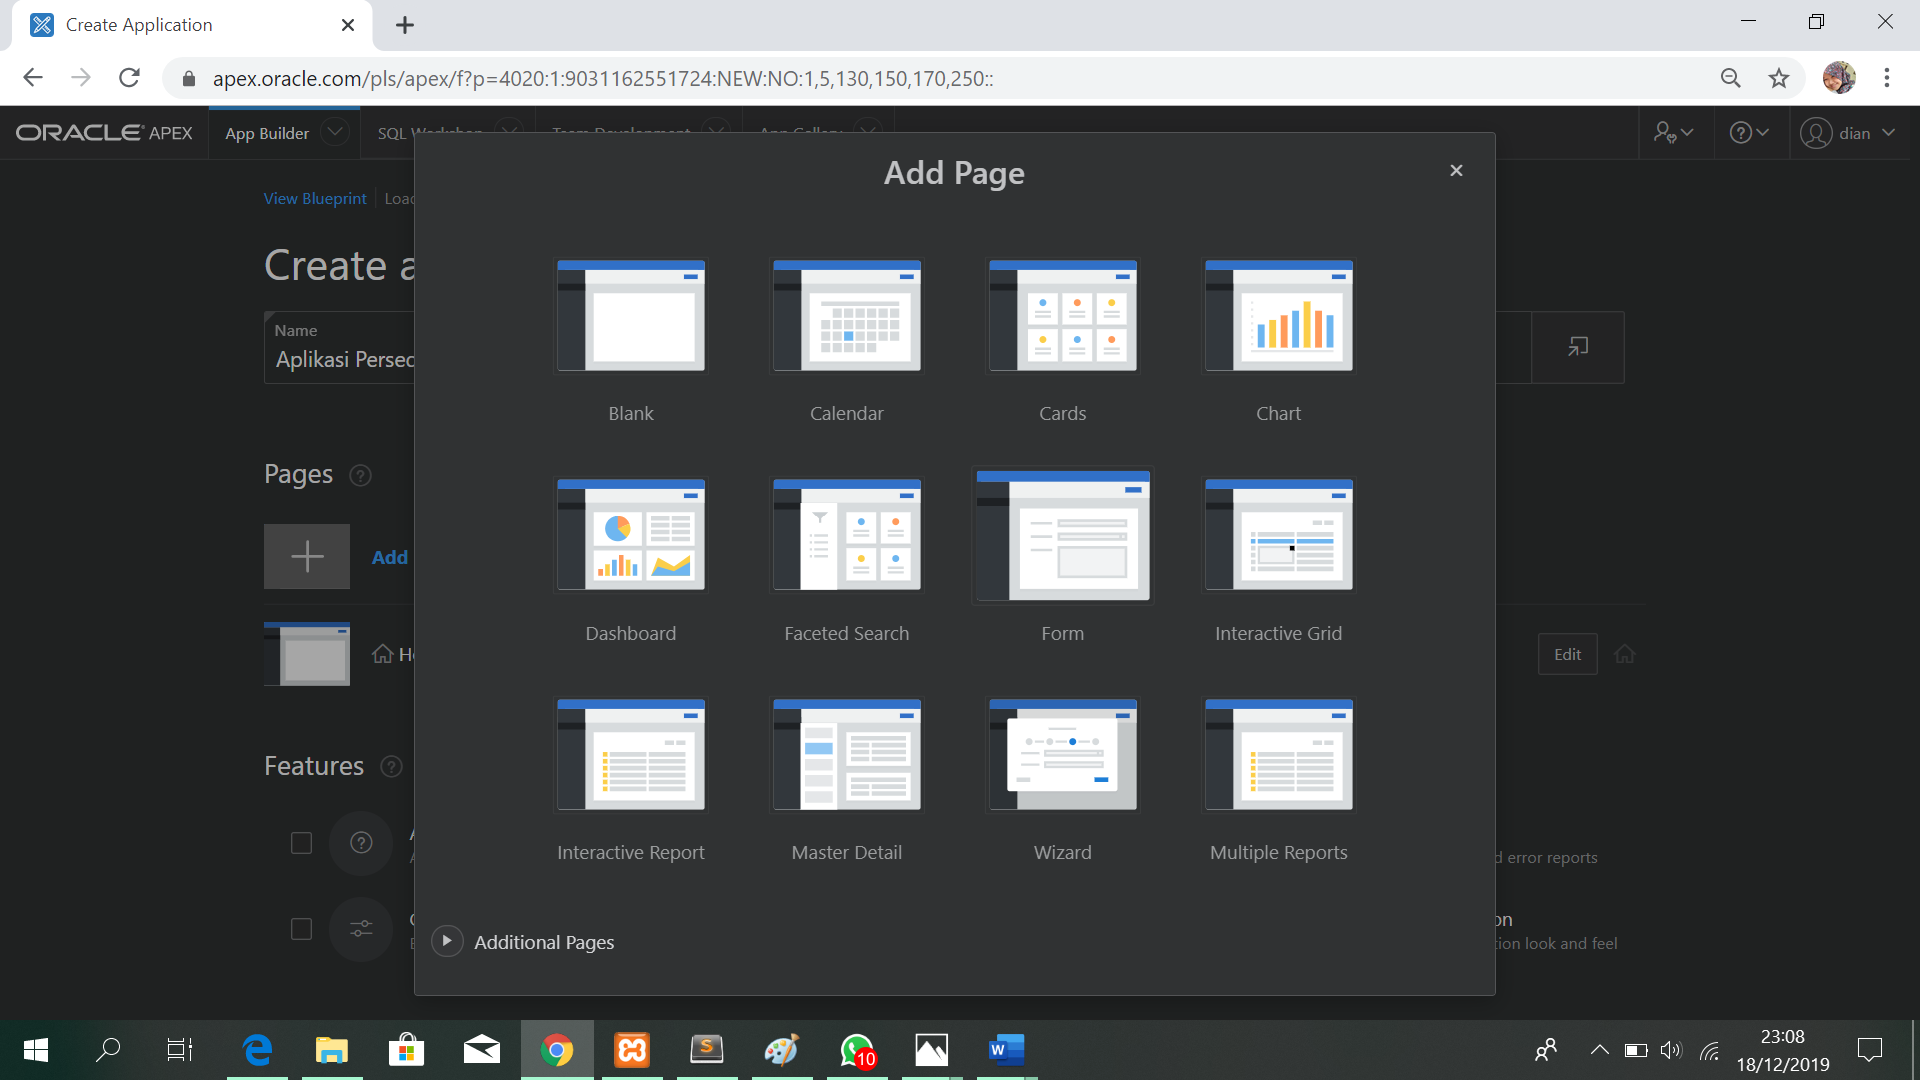
\includegraphics[width=13cm]{figure/4.png}
    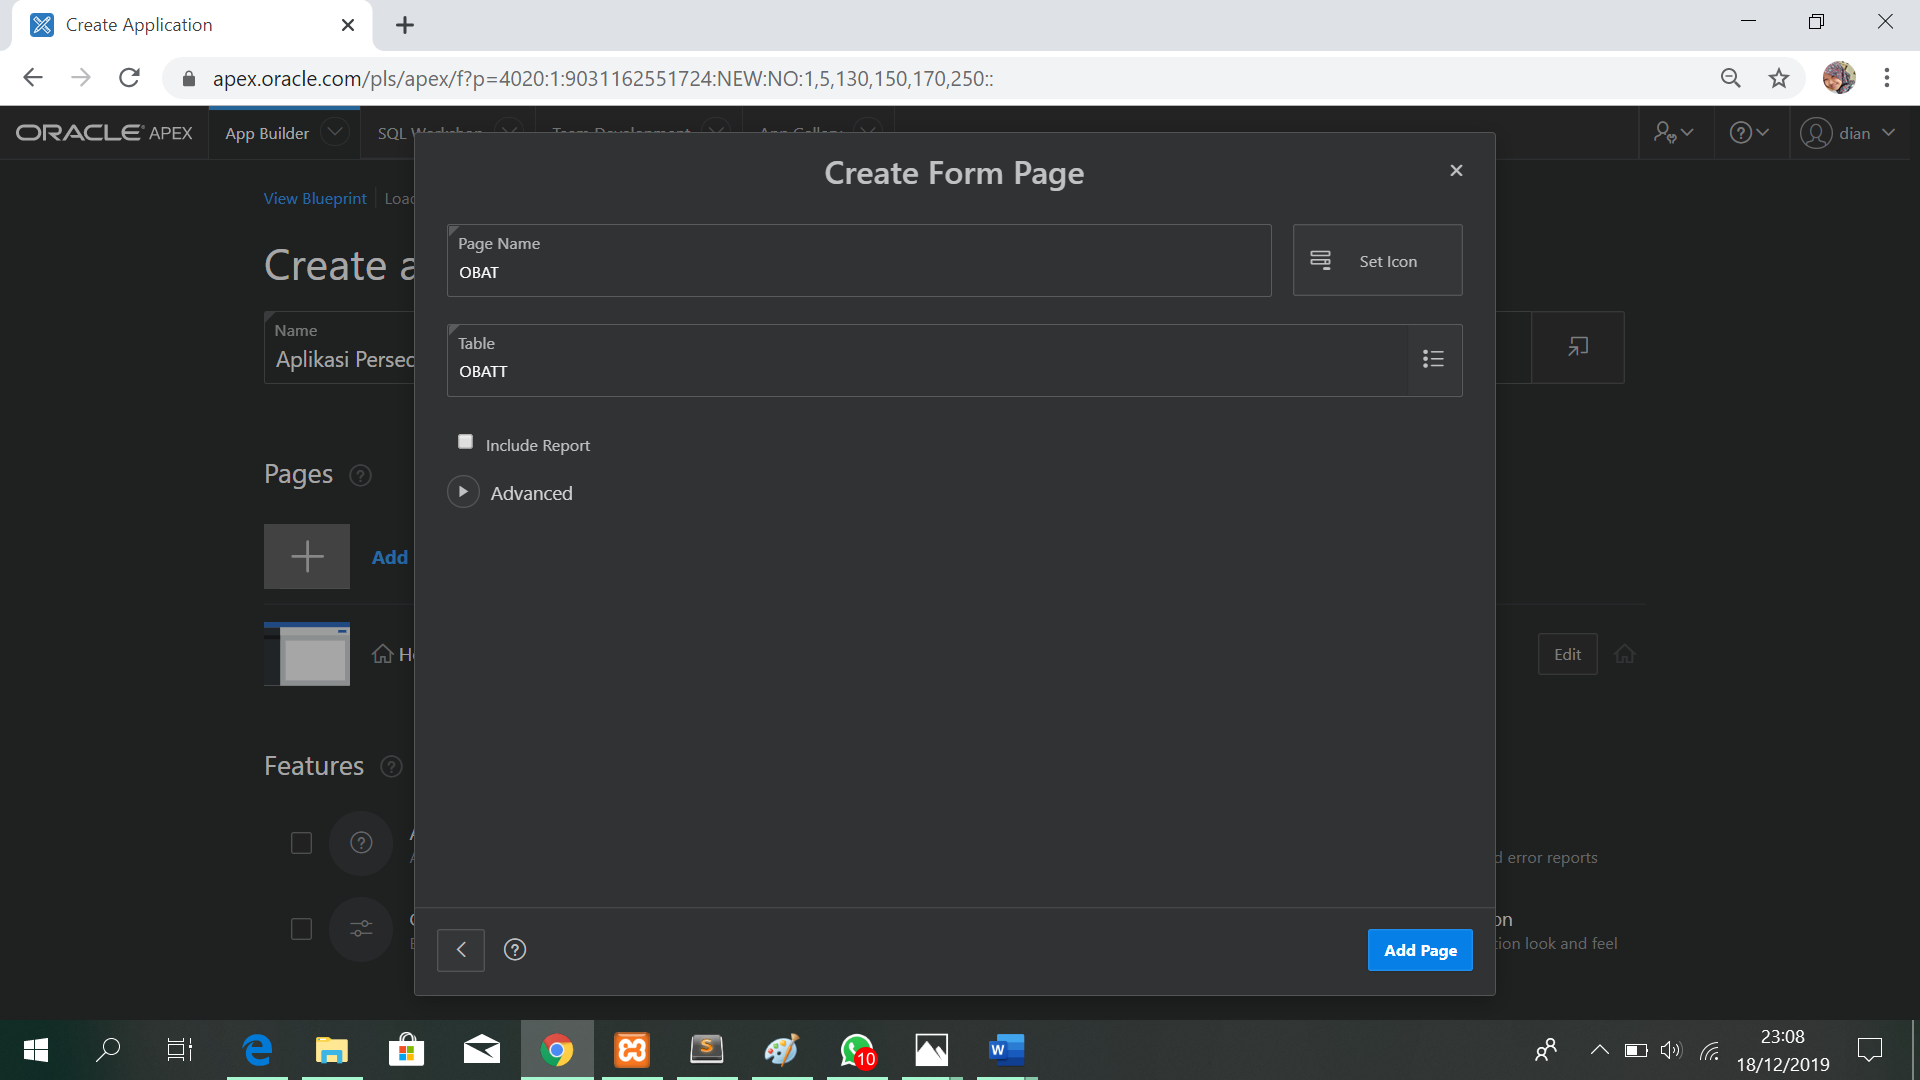
\includegraphics[width=13cm]{figure/5.png}
\end{center}
\\
5. jalankan aplikasi dengan pilih run application
\begin{center}
    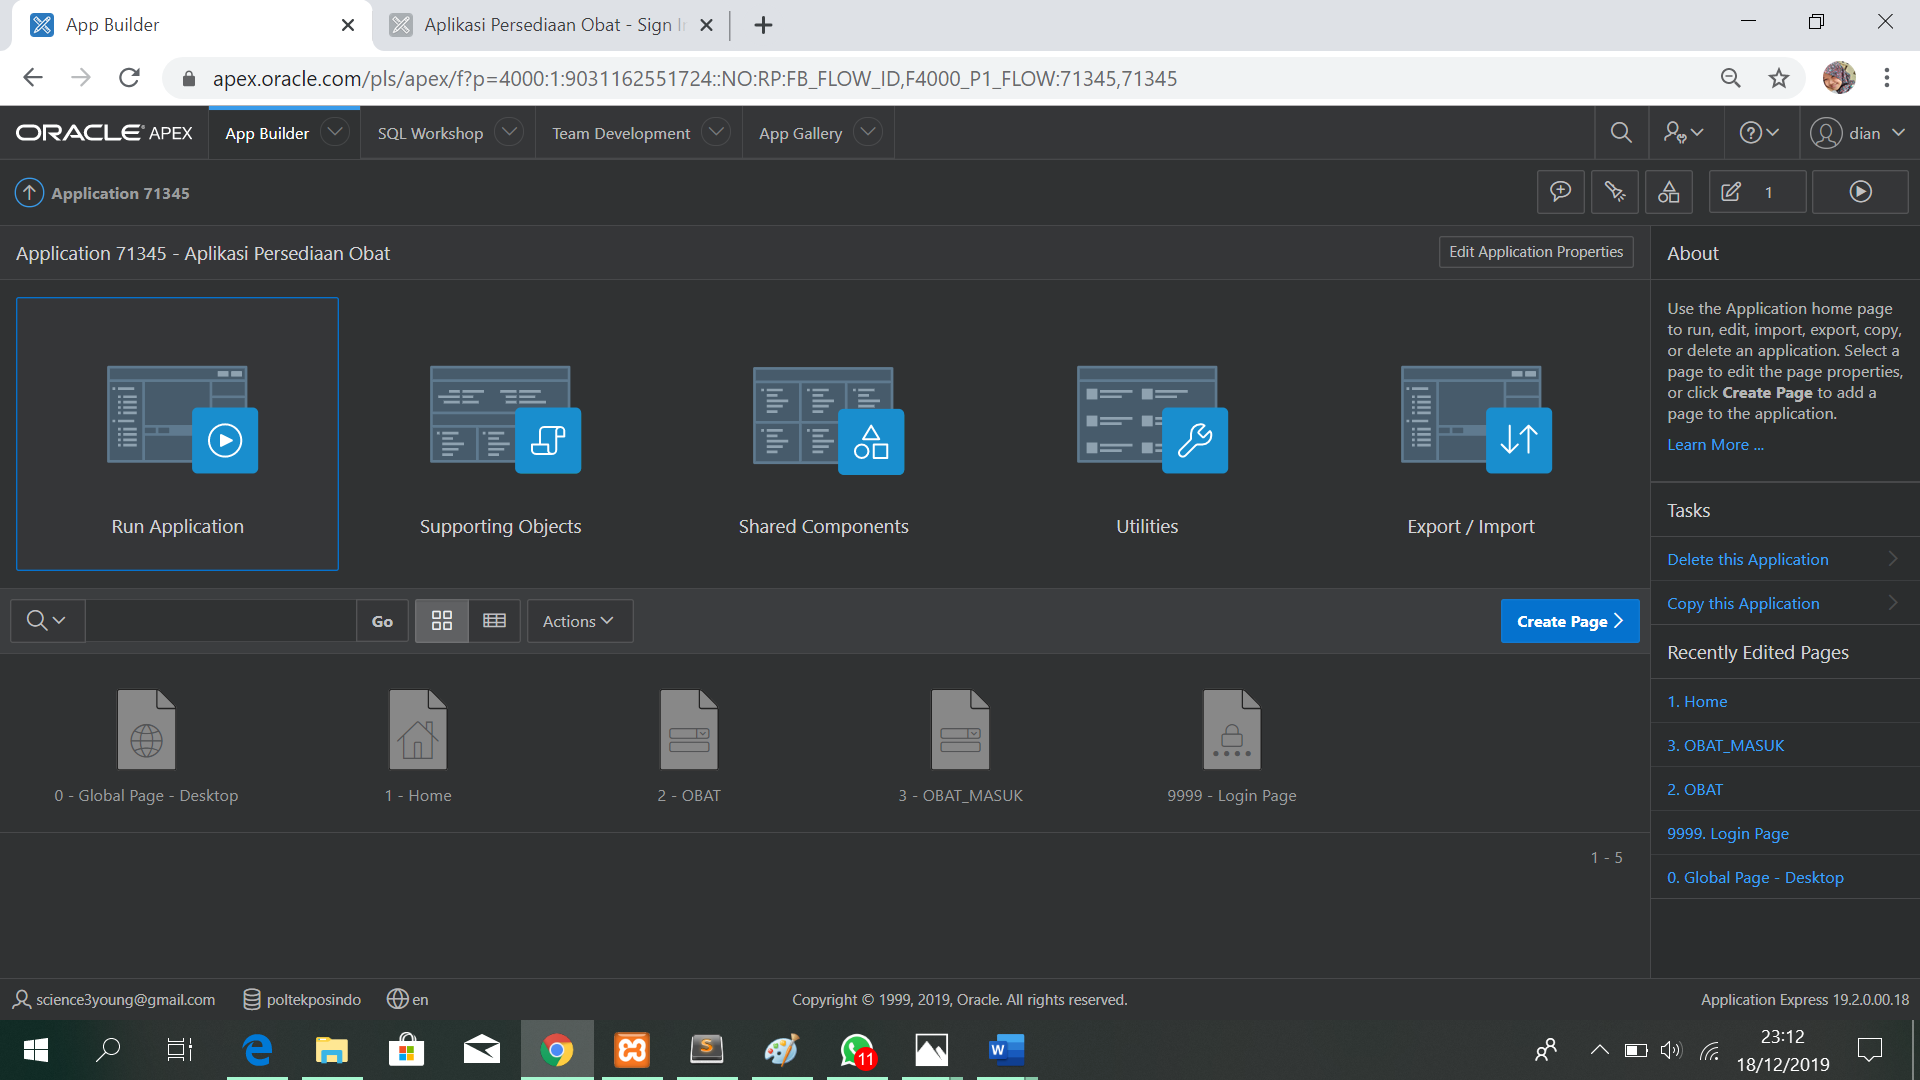
\includegraphics[width=13cm]{figure/7.png}
\end{center}
\\
6. Setelah berhasil Run Aplikasi, maka akan menampilkan login aplikasi. isi username dan password kemudian klik sign in
\begin{center}
    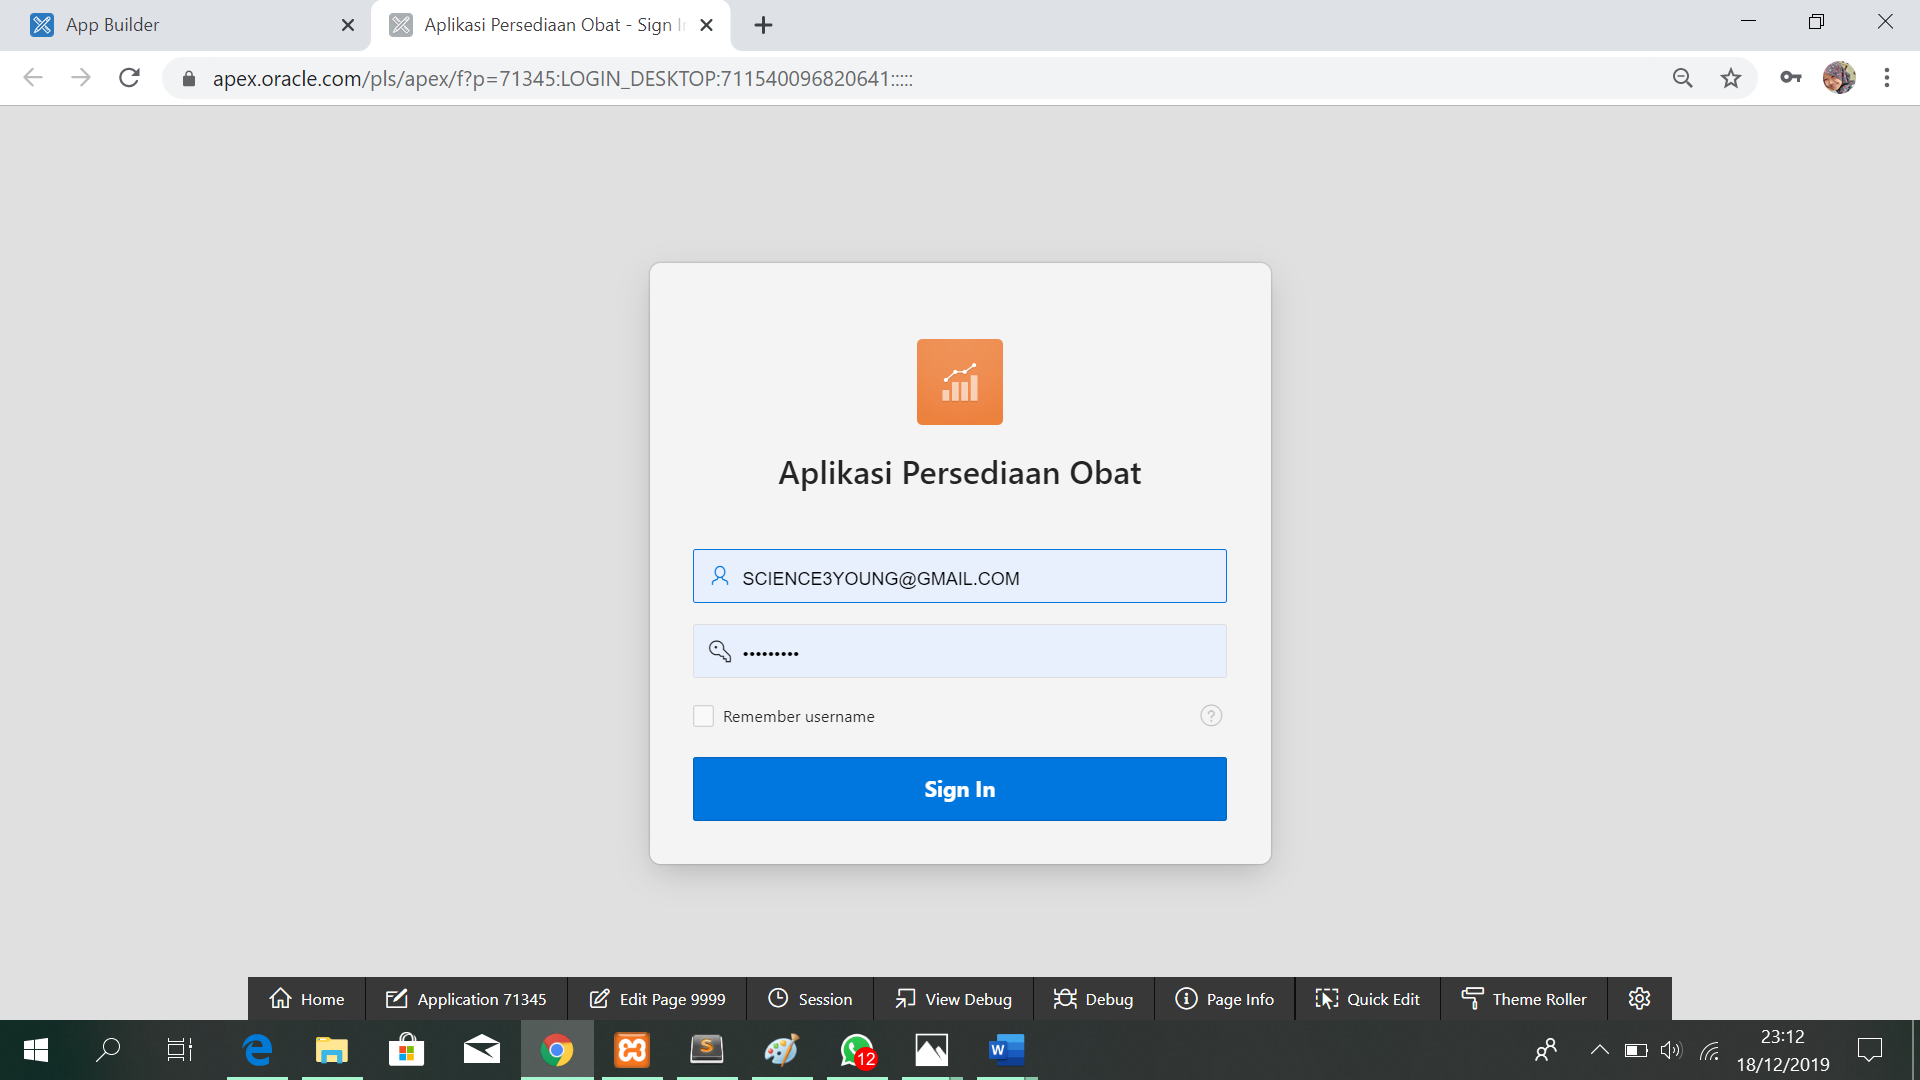
\includegraphics[width=13cm]{figure/8.png}
\end{center}
\\
7. Aplikasi Berhasil Dibuat.
\begin{center}
    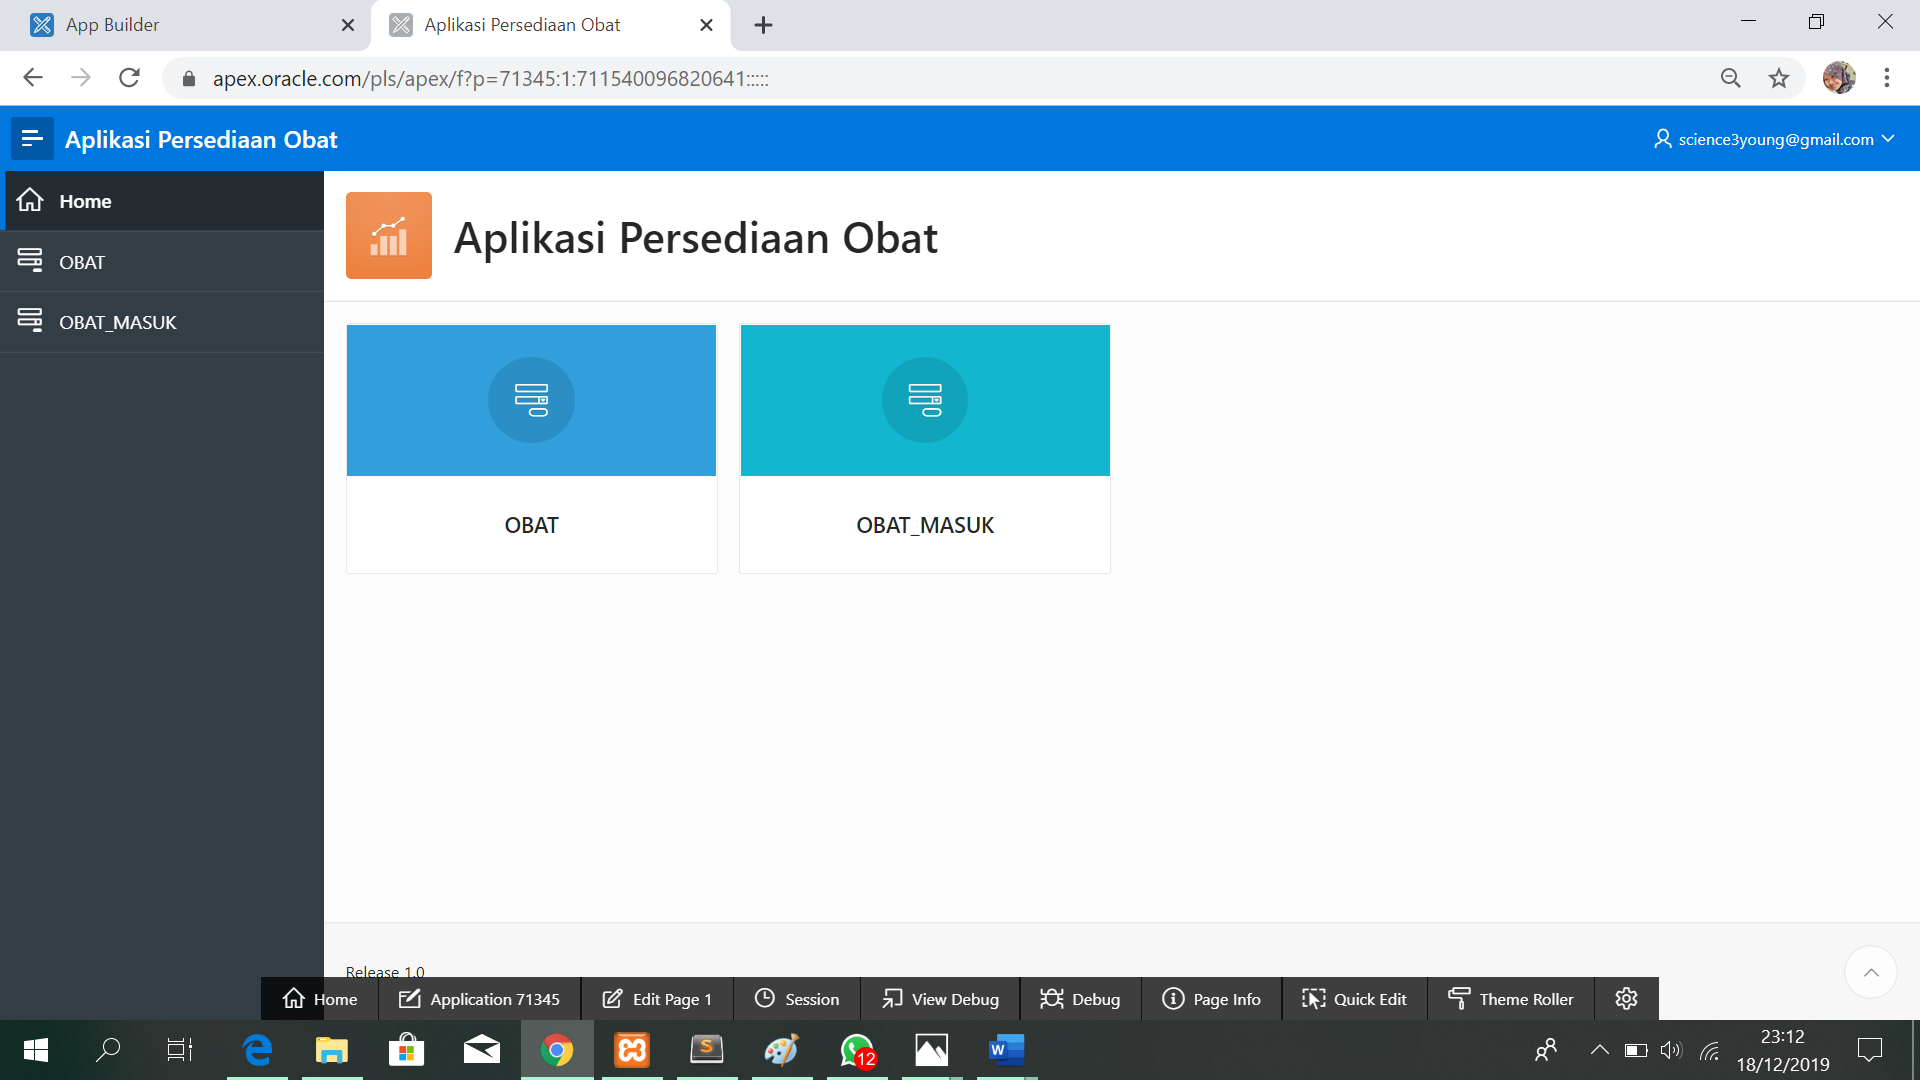
\includegraphics[width=13cm]{figure/9.png}
\end{center}
\\
Workspace: Poltekposindo\\
Username : science3young@gmail.com\\
password : dialine31\\
LINK: https://apex.oracle.com/pls/apex/f?p=4500:1000:116017521664752:::::











 


\end{document}
